\documentclass[problem]{mcs}

\begin{pcomments}
  \pcomment{spring07 pset4-8}
  \pcomment{slightly revised to not mention paths, by ARM 10/8/09}
\end{pcomments}

\pkeywords{
 graph theory
 induction
 buildup_error
 false_proof
}

\begin{problem}
Let's say that a graph has ``two ends'' if it has exactly two vertices
of degree 1 and all its other vertices have degree 2.  For example,
here is one such graph:
\begin{figure}[h]\redrawn

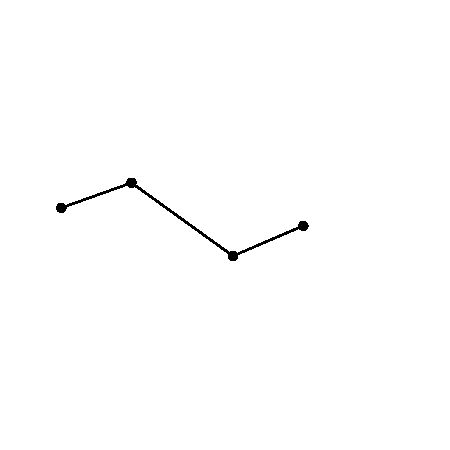
\includegraphics{ps4-path}

\end{figure}

\bparts

\ppart A \emph{line graph} is a graph whose vertices can be listed in a
sequence with edges between consecutive vertices only.  So the two-ended
graph above is also a line graph of length 4.

Prove that the following theorem is false by drawing a counterexample.

\begin{falsethm*}
Every two-ended graph is a line graph.
\end{falsethm*}

\begin{solution}A graph consisting of a path together with a simple cycle is a
counterexample.
\end{solution}

\ppart Point out the first erroneous statement in the following alleged
proof of the false theorem.  Describe the error as best you can.

\begin{falseproof}
We use induction.  The induction hypothesis is that every two-ended
graph with $n$ edges is a path.

\textbf{Base case ($n = 1$):} The only two-ended graph with a single edge
consists of two vertices joined by an edge:
\begin{figure}[h]\redrawn
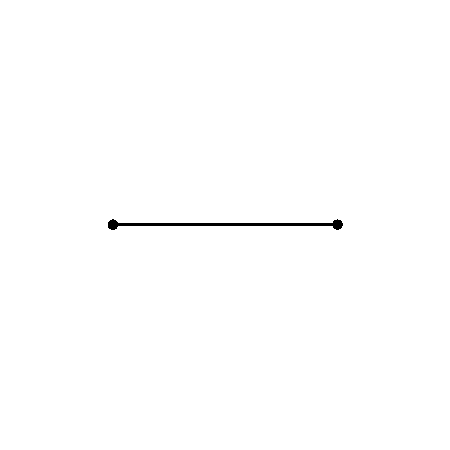
\includegraphics{ps4-oneedge}
\end{figure}

Sure enough, this is a line graph.

\textbf{Inductive case:} We assume that the induction hypothesis holds for
some $n \geq 1$ and prove that it holds for $n + 1$.  Let $G_n$ be any
two-ended graph with $n$ edges.  By the induction assumption, $G_n$ is a
line graph.  Now suppose that we create a two-ended graph $G_{n+1}$ by
adding one more edge to $G_n$.  This can be done in only one way: the new
edge must join an endpoint of $G_n$ to a new vertex; otherwise, $G_{n+1}$
would not be two-ended.
\begin{figure}[h]\redrawn
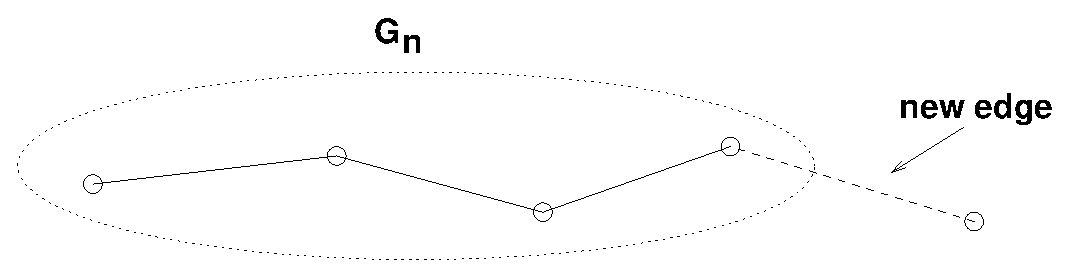
\includegraphics{ps4-induction}
\end{figure}

Clearly, $G_{n+1}$ is also a line graph.  Therefore, the induction
hypothesis holds for all graphs with $n+1$ edges, which completes the
proof by induction.

\end{falseproof}

\begin{solution}Actually, this is a correct proof of something else.  That is,
the first erroneous statement is the last one claiming that the 
induction hypothesis holds for \emph{all} $(n+1)$-edge two-ended
graphs.

The proof doesn't show this; rather, it only shows that the induction
hypothesis holds for those two-ended $(n+1)$-edge graphs {\em that can be
obtained by adding one more edge to an $n$-edge two-ended graph}.  This is
not all two-ended graphs, as the counterexample demonstrates.

This is an example of ``buildup'' error, where you assume that a size
$n+1$ object is built up in some particular way from similar objects of
smaller size.  (This assumption is correct for some kinds of objects, but
incorrect for others--- such as the one in the argument above.)

One way to avoid an accidental buildup error is to use a ``shrink down,
grow back'' process in the inductive step: start with a size $n+1$ object,
say a graph, remove a vertex (or edge), apply the inductive hypothesis
$P(n)$ to the smaller graph, and then add back the vertex (or edge) and
argue that $P(n+1)$ holds.  Let's see what would have happened if we'd
tried to prove the claim above by this method:

\textit{Inductive step:} We must show that $P(n)$ implies
$P(n+1)$ for all $n \geq 1$.  Consider an $(n+1)$-vertex graph $G$ in
which every vertex has degree at least 1.  Remove an arbitrary vertex
$v$, leaving an $n$-vertex graph $G'$ in which every vertex has
degree... uh-oh!

The reduced graph $G'$ might contain a vertex of degree 0, making the
inductive hypothesis $P(n)$ inapplicable!  We are stuck--- and
properly so, since the claim is false!
\end{solution}

\eparts

\end{problem}

